\batchmode
\documentclass[10pt]{book}
\RequirePackage{ifthen}


\usepackage{csvsimple}
\usepackage{booktabs}
\usepackage[shortlabels]{enumitem}
\usepackage[section]{placeins}
\usepackage{graphicx}
\usepackage{makeidx}
\usepackage{xintbinhex}
\usepackage{hang}
\usepackage[margin=1.0in]{geometry}
\usepackage[hyphens]{url}
\usepackage{multicol}
\usepackage{changepage}

\setlength{\parindent}{0pt} 

\setlength{\parskip}{6pt} 
\setlist{nosep}
\makeindex


\title{ZX Spectrum Next Programming Notes}
\date{\today}
\author{Theodore (Alex) Evans}%
\providecommand{\iis}{ I\textsuperscript{2}S }%
\providecommand{\iic}{ I\textsuperscript{2}C }%
\providecommand{\register}[3]{Register (#1) \$#2 (\xintHexToDec{#2}) $\Rightarrow$\  #3}%
\providecommand{\port}[2]{Port \$#1 (\xintHexToDec{#1}) #2}%
\providecommand{\textoverline}[1]{$\overline{\hbox{#1}}$}%
\providecommand{\sinset}{\end{multicols}\begin{adjustwidth}{0.05\textwidth}{0.05\textwidth}}%
\providecommand{\einset}{\end{adjustwidth}\begin{multicols}{2}} 


\usepackage{xcolor}

\usepackage[]{inputenc}



\makeatletter

\makeatletter
\count@=\the\catcode`\_ \catcode`\_=8 
\newenvironment{tex2html_wrap}{}{}%
\catcode`\<=12\catcode`\_=\count@
\newcommand{\providedcommand}[1]{\expandafter\providecommand\csname #1\endcsname}%
\newcommand{\renewedcommand}[1]{\expandafter\providecommand\csname #1\endcsname{}%
  \expandafter\renewcommand\csname #1\endcsname}%
\newcommand{\newedenvironment}[1]{\newenvironment{#1}{}{}\renewenvironment{#1}}%
\let\newedcommand\renewedcommand
\let\renewedenvironment\newedenvironment
\makeatother
\let\mathon=$
\let\mathoff=$
\ifx\AtBeginDocument\undefined \newcommand{\AtBeginDocument}[1]{}\fi
\newbox\sizebox
\setlength{\hoffset}{0pt}\setlength{\voffset}{0pt}
\addtolength{\textheight}{\footskip}\setlength{\footskip}{0pt}
\addtolength{\textheight}{\topmargin}\setlength{\topmargin}{0pt}
\addtolength{\textheight}{\headheight}\setlength{\headheight}{0pt}
\addtolength{\textheight}{\headsep}\setlength{\headsep}{0pt}
\setlength{\textwidth}{349pt}
\newwrite\lthtmlwrite
\makeatletter
\let\realnormalsize=\normalsize
\global\topskip=2sp
\def\preveqno{}\let\real@float=\@float \let\realend@float=\end@float
\def\@float{\let\@savefreelist\@freelist\real@float}
\def\liih@math{\ifmmode$\else\bad@math\fi}
\def\end@float{\realend@float\global\let\@freelist\@savefreelist}
\let\real@dbflt=\@dbflt \let\end@dblfloat=\end@float
\let\@largefloatcheck=\relax
\let\if@boxedmulticols=\iftrue
\def\@dbflt{\let\@savefreelist\@freelist\real@dbflt}
\def\adjustnormalsize{\def\normalsize{\mathsurround=0pt \realnormalsize
 \parindent=0pt\abovedisplayskip=0pt\belowdisplayskip=0pt}%
 \def\phantompar{\csname par\endcsname}\normalsize}%
\def\lthtmltypeout#1{{\let\protect\string \immediate\write\lthtmlwrite{#1}}}%
\usepackage[tightpage,active]{preview}
\newbox\lthtmlPageBox
\newdimen\lthtmlCropMarkHeight
\newdimen\lthtmlCropMarkDepth
\long\def\lthtmlTightVBox#1#2{%
    \setbox\lthtmlPageBox\vbox{\hbox{\catcode`\_=8 #2}}%
    \lthtmlCropMarkHeight=\ht\lthtmlPageBox \advance \lthtmlCropMarkHeight 6pt
    \lthtmlCropMarkDepth=\dp\lthtmlPageBox
    \lthtmltypeout{^^J:#1:lthtmlCropMarkHeight:=\the\lthtmlCropMarkHeight}%
    \lthtmltypeout{^^J:#1:lthtmlCropMarkDepth:=\the\lthtmlCropMarkDepth:1ex:=\the \dimexpr 1ex}%
    \begin{preview}\copy\lthtmlPageBox\end{preview}}}%
\long\def\lthtmlTightFBox#1#2{%
    \adjustnormalsize\setbox\lthtmlPageBox=\vbox\bgroup %
    \let\ifinner=\iffalse \let\)\liih@math %
    {\catcode`\_=8 #2}%
    \@next\next\@currlist{}{\def\next{\voidb@x}}%
    \expandafter\box\next\egroup %
    \lthtmlCropMarkHeight=\ht\lthtmlPageBox \advance \lthtmlCropMarkHeight 6pt
    \lthtmlCropMarkDepth=\dp\lthtmlPageBox
    \lthtmltypeout{^^J:#1:lthtmlCropMarkHeight:=\the\lthtmlCropMarkHeight}%
    \lthtmltypeout{^^J:#1:lthtmlCropMarkDepth:=\the\lthtmlCropMarkDepth:1ex:=\the \dimexpr 1ex}%
    \begin{preview}\copy\lthtmlPageBox\end{preview}}%
    \long\def\lthtmlinlinemathA#1#2\lthtmlindisplaymathZ{\lthtmlTightVBox{#1}{#2}}
    \def\lthtmlinlineA#1#2\lthtmlinlineZ{\lthtmlTightVBox{#1}{#2}}
    \long\def\lthtmldisplayA#1#2\lthtmldisplayZ{\lthtmlTightVBox{#1}{#2}}
    \long\def\lthtmlinlinemathA#1#2\lthtmlindisplaymathZ{\lthtmlTightVBox{#1}{#2}}
    \def\lthtmlinlineA#1#2\lthtmlinlineZ{\lthtmlTightVBox{#1}{#2}}
    \long\def\lthtmldisplayA#1#2\lthtmldisplayZ{\lthtmlTightVBox{#1}{#2}}
    \long\def\lthtmldisplayB#1#2\lthtmldisplayZ{\\edef\preveqno{(\theequation)}%
        \lthtmlTightVBox{#1}{\let\@eqnnum\relax#2}}
    \long\def\lthtmlfigureA#1#2\lthtmlfigureZ{\let\@savefreelist\@freelist
        \lthtmlTightFBox{#1}{#2}\global\let\@freelist\@savefreelist}
    \long\def\lthtmlpictureA#1#2\lthtmlpictureZ{\let\@savefreelist\@freelist
        \lthtmlTightVBox{#1}{#2}\global\let\@freelist\@savefreelist}
\def\lthtmlcheckvsize{\ifdim\ht\sizebox<\vsize 
  \ifdim\wd\sizebox<\hsize\expandafter\hfill\fi \expandafter\vfill
  \else\expandafter\vss\fi}%
\providecommand{\selectlanguage}[1]{}%
\makeatletter \tracingstats = 1 


\begin{document}
\pagestyle{empty}\thispagestyle{empty}\lthtmltypeout{}%
\lthtmltypeout{latex2htmlLength hsize=\the\hsize}\lthtmltypeout{}%
\lthtmltypeout{latex2htmlLength vsize=\the\vsize}\lthtmltypeout{}%
\lthtmltypeout{latex2htmlLength hoffset=\the\hoffset}\lthtmltypeout{}%
\lthtmltypeout{latex2htmlLength voffset=\the\voffset}\lthtmltypeout{}%
\lthtmltypeout{latex2htmlLength topmargin=\the\topmargin}\lthtmltypeout{}%
\lthtmltypeout{latex2htmlLength topskip=\the\topskip}\lthtmltypeout{}%
\lthtmltypeout{latex2htmlLength headheight=\the\headheight}\lthtmltypeout{}%
\lthtmltypeout{latex2htmlLength headsep=\the\headsep}\lthtmltypeout{}%
\lthtmltypeout{latex2htmlLength parskip=\the\parskip}\lthtmltypeout{}%
\lthtmltypeout{latex2htmlLength oddsidemargin=\the\oddsidemargin}\lthtmltypeout{}%
\makeatletter
\if@twoside\lthtmltypeout{latex2htmlLength evensidemargin=\the\evensidemargin}%
\else\lthtmltypeout{latex2htmlLength evensidemargin=\the\oddsidemargin}\fi%
\lthtmltypeout{}%
\makeatother
\setcounter{page}{1}
\onecolumn

% !!! IMAGES START HERE !!!

{\newpage\clearpage
\lthtmlinlinemathA{tex2html_wrap_inline8081}%
$256\times 192$%
\lthtmlindisplaymathZ
\lthtmlcheckvsize\clearpage}

{\newpage\clearpage
\lthtmlinlinemathA{tex2html_wrap_inline8087}%
$320\times 256$%
\lthtmlindisplaymathZ
\lthtmlcheckvsize\clearpage}

{\newpage\clearpage
\lthtmlinlinemathA{tex2html_wrap_inline8090}%
$640\times 256$%
\lthtmlindisplaymathZ
\lthtmlcheckvsize\clearpage}

\stepcounter{chapter}
\stepcounter{chapter}
\stepcounter{section}
\stepcounter{subsection}
{\newpage\clearpage
\lthtmlinlinemathA{tex2html_wrap_inline103}%
$256\times192\times256$%
\lthtmlindisplaymathZ
\lthtmlcheckvsize\clearpage}

{\newpage\clearpage
\lthtmlinlinemathA{tex2html_wrap_inline105}%
$320\times256\times256$%
\lthtmlindisplaymathZ
\lthtmlcheckvsize\clearpage}

{\newpage\clearpage
\lthtmlinlinemathA{tex2html_wrap_inline107}%
$640\times256\times6$%
\lthtmlindisplaymathZ
\lthtmlcheckvsize\clearpage}

{\newpage\clearpage
\lthtmlinlinemathA{tex2html_wrap_inline126}%
$\Rightarrow$%
\lthtmlindisplaymathZ
\lthtmlcheckvsize\clearpage}

\stepcounter{subsection}
\stepcounter{paragraph}
\stepcounter{subsection}
\stepcounter{subsection}
\stepcounter{section}
\stepcounter{subsection}
\stepcounter{paragraph}
{\newpage\clearpage
\lthtmlfigureA{adjustwidth258}%
\begin{adjustwidth}
% latex2html id marker 258
{0.05\textwidth}{0.05\textwidth}
\begin{table}[h]\centering
  \caption{ULA Colour}
  \csvautotabular{video/flash.csv}
\end{table}
\end{adjustwidth}%
\lthtmlfigureZ
\lthtmlcheckvsize\clearpage}

\stepcounter{paragraph}
{\newpage\clearpage
\lthtmlfigureA{adjustwidth265}%
\begin{adjustwidth}
% latex2html id marker 265
{0.05\textwidth}{0.05\textwidth}
\begin{table}[h]\centering
  \caption{ULA Next}
  \csvautotabular{video/palfmt.csv}
\end{table}
\end{adjustwidth}%
\lthtmlfigureZ
\lthtmlcheckvsize\clearpage}

\stepcounter{paragraph}
\stepcounter{subparagraph}
\stepcounter{subparagraph}
\stepcounter{subparagraph}
\stepcounter{subparagraph}
\stepcounter{subparagraph}
\stepcounter{subparagraph}
{\newpage\clearpage
\lthtmlfigureA{adjustwidth272}%
\begin{adjustwidth}{0.05\textwidth}{0.05\textwidth}
\begin{verbatim}

; 64 colour palette file format (internal) - version 1.0
; copyright (c) 2009 Andrew Owen
;
; The palette file is stored as a BASIC program with embedded machine code

header:

db 0x00 ; program file
db 0x14, 0x01, "64colour" ; file name
dw 0x0097 ; data length
dw 0x0000 ; autostart line
dw 0x0097 ; program length

basic:

; 0 RANDOMIZE USR ((PEEK VAL "2
; 3635"+VAL "256"*PEEK VAL "23636"
; )+VAL "48"): LOAD "": REM

db 0x00, 0x00, 0x93, 0x00, 0xf9, 0xc0, 0x28, 0x28
db 0xbe, 0xb0, 0x22, 0x32, 0x33, 0x36, 0x33, 0x35
db 0x22, 0x2b, 0xb0, 0x22, 0x32, 0x35, 0x36, 0x22
db 0x2a, 0xbe, 0xb0, 0x22, 0x32, 0x33, 0x36, 0x33
db 0x36, 0x22, 0x29, 0x2b, 0xb0, 0x22, 0x34, 0x38
db 0x22, 0x29, 0x3a, 0xef, 0x22, 0x22, 0x3a, 0xea

start:

di ; disable interrupts
ld hl, 38 ; HL = length of code
add hl, bc ; BC = entry point (start) from BASIC
ld bc, 0xbf3b ; register select
ld a, 64 ; mode group
out (c), a ;
ld a, 1 ;
ld b, 0xff ; choose register port
out (c), a ; turn palette mode on
xor a ; first register

setreg:

ld b, 0xbf ; choose register port
out (c), a ; select register
ex af, af' ; save current register select
ld a, (hl) ; get data
ld b, 0xff ; choose data port
out (c), a ; set it
ex af, af' ; restore current register
inc hl ; advance pointer
inc a ; increase register
cp 64 ; are we nearly there yet?
jr nz, setreg ; repeat until all 64 have been done
ei ; enable interrupts
ret ; return

; this is where the actual data is stored. The following is an example palette.

registers:

db 0x00, 0x02, 0x18, 0x1b, 0xc0, 0xc3, 0xd8, 0xdb ; INK
db 0x00, 0x02, 0x18, 0x1b, 0xc0, 0xc3, 0xd8, 0xdb ; PAPER
db 0x00, 0x03, 0x1c, 0x1f, 0xe0, 0xe3, 0xfc, 0xff ; +BRIGHT
db 0x00, 0x03, 0x1c, 0x1f, 0xe0, 0xe3, 0xfc, 0xff ;
db 0xdb, 0xd8, 0xc3, 0xc0, 0x1b, 0x18, 0x02, 0x00 ; +FLASH
db 0xdb, 0xd8, 0xc3, 0xc0, 0x1b, 0x18, 0x02, 0x00 ;
db 0xff, 0xfc, 0xe3, 0xe0, 0x1f, 0x1c, 0x03, 0x00 ; +BRIGHT/
db 0xff, 0xfc, 0xe3, 0xe0, 0x1f, 0x1c, 0x03, 0x00 ; +FLASH

terminating_byte:

db 0x0d\end{verbatim}

\end{adjustwidth}%
\lthtmlfigureZ
\lthtmlcheckvsize\clearpage}

\stepcounter{subsection}
\stepcounter{subsection}
\stepcounter{subsection}
{\newpage\clearpage
\lthtmlinlinemathA{tex2html_wrap_inline443}%
$8\times8$%
\lthtmlindisplaymathZ
\lthtmlcheckvsize\clearpage}

{\newpage\clearpage
\lthtmlinlinemathA{tex2html_wrap_inline445}%
$32\times24$%
\lthtmlindisplaymathZ
\lthtmlcheckvsize\clearpage}

{\newpage\clearpage
\lthtmlinlinemathA{tex2html_wrap_inline455}%
$0R_4R_3Y_2Y_1Y_0R_2R_1R_0C_4C_3C_2C_1C_0$%
\lthtmlindisplaymathZ
\lthtmlcheckvsize\clearpage}

{\newpage\clearpage
\lthtmlinlinemathA{tex2html_wrap_inline459}%
$0110R_4R_3R_2R_1R_0C_4C_3C_2C_1C_0$%
\lthtmlindisplaymathZ
\lthtmlcheckvsize\clearpage}

{\newpage\clearpage
\lthtmlfigureA{adjustwidth405}%
\begin{adjustwidth}{0.05\textwidth}{0.05\textwidth}
Code:
\begin{verbatim}

;; from any other Timex mode:
ld a,$00
ld c,$ff
out (c),a

;; from LoRes mode:
ld bc,$243B ; next register select port
ld a,$15
out (c),a
ld bc,$253B ; next register r/w port
in a,(c)
and $7f
out (c),a\end{verbatim}

\end{adjustwidth}%
\lthtmlfigureZ
\lthtmlcheckvsize\clearpage}

\stepcounter{subsection}
{\newpage\clearpage
\lthtmlinlinemathA{tex2html_wrap_inline461}%
$1R_4R_3Y_2Y_1Y_0R_2R_1R_0C_4C_3C_2C_1C_0$%
\lthtmlindisplaymathZ
\lthtmlcheckvsize\clearpage}

{\newpage\clearpage
\lthtmlinlinemathA{tex2html_wrap_inline463}%
$1110R_4R_3R_2R_1R_0C_4C_3C_2C_1C_0$%
\lthtmlindisplaymathZ
\lthtmlcheckvsize\clearpage}

{\newpage\clearpage
\lthtmlfigureA{adjustwidth412}%
\begin{adjustwidth}{0.05\textwidth}{0.05\textwidth}
Code:
\par
\begin{verbatim}

;; disable LoRes mode:
ld bc,$243B ; next register select port
ld a,$15
out (c),a
ld bc,$253B ; next register r/w port
in a,(c)
and $7f
out (c),a
;; set Timex mode
ld bc,$243B ; next register select port
ld a,$08
out (c),a
ld bc,$253B ; next register r/w port
in a,(c)
or $04
out (c),a
;; set alternate page mode
ld c,$ff
ld a,$01
out (c),a\end{verbatim}

\end{adjustwidth}%
\lthtmlfigureZ
\lthtmlcheckvsize\clearpage}

\stepcounter{subsection}
{\newpage\clearpage
\lthtmlinlinemathA{tex2html_wrap_inline467}%
$8\times1$%
\lthtmlindisplaymathZ
\lthtmlcheckvsize\clearpage}

{\newpage\clearpage
\lthtmlinlinemathA{tex2html_wrap_inline469}%
$32\times192$%
\lthtmlindisplaymathZ
\lthtmlcheckvsize\clearpage}

{\newpage\clearpage
\lthtmlfigureA{adjustwidth419}%
\begin{adjustwidth}{0.05\textwidth}{0.05\textwidth}
Code:
\begin{verbatim}

;; disable LoRes mode:
ld bc,$243B ; next register select port
ld a,$15
out (c),a
ld bc,$253B ; next register r/w port
in a,(c)
and $7f
out (c),a
;; set Timex mode
ld bc,$243B ; next register select port
ld a,$08
out (c),a
ld bc,$253B ; next register r/w port
in a,(c)
or $04
out (c),a
;; set hi-colour mode
ld c,$ff
ld a,$02
out (c),a\end{verbatim}

\end{adjustwidth}%
\lthtmlfigureZ
\lthtmlcheckvsize\clearpage}

\stepcounter{subsection}
{\newpage\clearpage
\lthtmlinlinemathA{tex2html_wrap_inline477}%
$512\times192$%
\lthtmlindisplaymathZ
\lthtmlcheckvsize\clearpage}

{\newpage\clearpage
\lthtmlfigureA{adjustwidth426}%
\begin{adjustwidth}
% latex2html id marker 426
{0.05\textwidth}{0.05\textwidth}
\begin{table}[h]\centering
  \caption{Hi-Resolution Colours}
  \csvautotabular{video/hires.csv}
\end{table}
\end{adjustwidth}%
\lthtmlfigureZ
\lthtmlcheckvsize\clearpage}

{\newpage\clearpage
\lthtmlinlinemathA{tex2html_wrap_inline479}%
$64\times32$%
\lthtmlindisplaymathZ
\lthtmlcheckvsize\clearpage}

{\newpage\clearpage
\lthtmlinlinemathA{tex2html_wrap_inline483}%
$64\times24$%
\lthtmlindisplaymathZ
\lthtmlcheckvsize\clearpage}

{\newpage\clearpage
\lthtmlinlinemathA{tex2html_wrap_inline485}%
$C_0R_4R_3Y_2Y_1Y_0R_2R_1R_0C_5C_4C_3C_2C_1$%
\lthtmlindisplaymathZ
\lthtmlcheckvsize\clearpage}

{\newpage\clearpage
\lthtmlfigureA{adjustwidth433}%
\begin{adjustwidth}{0.05\textwidth}{0.05\textwidth}
Code:
\begin{verbatim}

;; disable LoRes mode:
ld bc,$243B ; next register select port
ld a,$15
out (c),a
ld bc,$253B ; next register r/w port
in a,(c)
and $7f
out (c),a
;; set Timex mode
ld bc,$243B ; next register select port
ld a,$08
out (c),a
ld bc,$253B ; next register r/w port
in a,(c)
or $04
out (c),a
;; set hi-res mode, black on white
ld c,$ff
ld a,$06
out (c),a\end{verbatim}

\end{adjustwidth}%
\lthtmlfigureZ
\lthtmlcheckvsize\clearpage}

\stepcounter{subsection}
{\newpage\clearpage
\lthtmlinlinemathA{tex2html_wrap_inline487}%
$128\times96$%
\lthtmlindisplaymathZ
\lthtmlcheckvsize\clearpage}

{\newpage\clearpage
\lthtmlinlinemathA{tex2html_wrap_inline489}%
$100xxxxx$%
\lthtmlindisplaymathZ
\lthtmlcheckvsize\clearpage}

{\newpage\clearpage
\lthtmlfigureA{adjustwidth576}%
\begin{adjustwidth}{0.05\textwidth}{0.05\textwidth}
Code: 256 colour
\begin{verbatim}

;; enable LoRes mode:
nextreg $15,$80
;; 256-colour mode
ld bc,$243B ; next register select port
ld a,$6A
out (c),a
ld bc,$253B ; next register r/w port
in a,(c)
and $EF ; lores radistan control
out (c),a\end{verbatim}

\par
Code: 16 colour
\begin{verbatim}

;; enable LoRes mode:
nextreg $15,$80
;; 16-colour mode
nextreg $6A,$10\end{verbatim}

\end{adjustwidth}%
\lthtmlfigureZ
\lthtmlcheckvsize\clearpage}

\stepcounter{section}
{\newpage\clearpage
\lthtmlinlinemathA{tex2html_wrap_inline596}%
$640\times256\times16$%
\lthtmlindisplaymathZ
\lthtmlcheckvsize\clearpage}

\stepcounter{subsection}
\stepcounter{paragraph}
\stepcounter{paragraph}
\stepcounter{paragraph}
\stepcounter{paragraph}
\stepcounter{subsection}
\stepcounter{subsection}
\stepcounter{section}
\stepcounter{subsection}
{\newpage\clearpage
\lthtmlinlinemathA{tex2html_wrap_inline740}%
$40\times32$%
\lthtmlindisplaymathZ
\lthtmlcheckvsize\clearpage}

{\newpage\clearpage
\lthtmlinlinemathA{tex2html_wrap_inline744}%
$80\times32$%
\lthtmlindisplaymathZ
\lthtmlcheckvsize\clearpage}

{\newpage\clearpage
\lthtmlinlinemathA{tex2html_wrap_inline750}%
$40\times30$%
\lthtmlindisplaymathZ
\lthtmlcheckvsize\clearpage}

{\newpage\clearpage
\lthtmlinlinemathA{tex2html_wrap_inline752}%
$80\times30$%
\lthtmlindisplaymathZ
\lthtmlcheckvsize\clearpage}

\stepcounter{subsection}
\stepcounter{paragraph}
\stepcounter{paragraph}
\stepcounter{subsection}
\stepcounter{subsection}
\stepcounter{subsection}
\stepcounter{paragraph}
\stepcounter{paragraph}
\stepcounter{section}
{\newpage\clearpage
\lthtmlinlinemathA{tex2html_wrap_inline1045}%
$16\times16$%
\lthtmlindisplaymathZ
\lthtmlcheckvsize\clearpage}

{\newpage\clearpage
\lthtmlinlinemathA{tex2html_wrap_inline1047}%
$2\times$%
\lthtmlindisplaymathZ
\lthtmlcheckvsize\clearpage}

{\newpage\clearpage
\lthtmlinlinemathA{tex2html_wrap_inline1049}%
$4\times$%
\lthtmlindisplaymathZ
\lthtmlcheckvsize\clearpage}

{\newpage\clearpage
\lthtmlinlinemathA{tex2html_wrap_inline1051}%
$8\times$%
\lthtmlindisplaymathZ
\lthtmlcheckvsize\clearpage}

\stepcounter{subsection}
\stepcounter{paragraph}
\stepcounter{subparagraph}
{\newpage\clearpage
\lthtmlfigureA{adjustwidth1030}%
\begin{adjustwidth}
% latex2html id marker 1030
{0.05\textwidth}{0.05\textwidth}
As an example of an 8-bit sprite, let’s have a look at figure 2.1.
\par
\begin{figure}\centering
  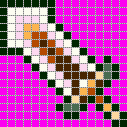
\includegraphics{video/sprite_1.png}
  \caption{Pattern Example}
\end{figure}
\par
Using the default palette, which is initialised with RGB332 colours
from 0-255, the hexadecimal values for this pattern arranged in a
$16\times16$\  array are shown below:
\par
\begin{verbatim}

04040404040404E3E3E3E3E3E3E3E3E3
04FFFFFFFFFF04E3E3E3E3E3E3E3E3E3
04FFFBFBFBFF04E3E3E3E3E3E3E3E3E3
04FFFBF5F5FBFF04E3E3E3E3E3E3E3E3
04FFFBF5A8A8FBFF04E3E3E3E3E3E3E3
04FFFFFBA844A8FBFF04E3E3E3E3E3E3
040404FFFBA844A8FBFF04E3E3E3E3E3
E3E3E304FFFBA84444FBFF04E304E3E3
E3E3E3E304FFFB444444FBFF044D04E3
E3E3E3E3E304FFFB44444444FA4D04E3
E3E3E3E3E3E304FFFB44FFF54404E3E3
E3E3E3E3E3E3E304FF44F5A804E3E3E3
E3E3E3E3E3E3E3E304FA4404A804E3E3
E3E3E3E3E3E3E3044D4D04E304F504E3
E3E3E3E3E3E3E3E30404E3E3E304FA04
E3E3E3E3E3E3E3E3E3E3E3E3E3E30404\end{verbatim}

\par
Here \$E3 is used as the transparent index.
\par
These 256 bytes would be stored in pattern memory in left to right,
top to bottom order.
\end{adjustwidth}%
\lthtmlfigureZ
\lthtmlcheckvsize\clearpage}

\stepcounter{subparagraph}
{\newpage\clearpage
\lthtmlfigureA{adjustwidth1037}%
\begin{adjustwidth}{0.05\textwidth}{0.05\textwidth}
As an example we will use the same sprite image as was given in the
8-bit pattern example. Here only the lower 4 bits of each pixel is
retained to confine each pixel’s color to 4-bits:
\par
\begin{verbatim}

4444444333333333
4FFFFF4333333333
4FBBBF4333333333
4FB55BF433333333
4FB588BF43333333
4FFB848BF4333333
444FB848BF433333
3334FB844BF43433
33334FB444BF4D43
333334FB4444AD43
3333334FB4F54433
33333334F4584333
333333334A448433
33333334DD434543
33333333443334A4
3333333333333344\end{verbatim}

\par
\$3 is used as the transparent index.
\par
These 128 bytes would be stored in pattern memory in left to right,
top to bottom order.
\end{adjustwidth}%
\lthtmlfigureZ
\lthtmlcheckvsize\clearpage}

\stepcounter{subsection}
\stepcounter{subsection}
{\newpage\clearpage
\lthtmlinlinemathA{tex2html_wrap_inline1073}%
$1\times$%
\lthtmlindisplaymathZ
\lthtmlcheckvsize\clearpage}

{\newpage\clearpage
\lthtmlinlinemathA{tex2html_wrap_inline1077}%
$4\times4$%
\lthtmlindisplaymathZ
\lthtmlcheckvsize\clearpage}

\stepcounter{subsection}
\stepcounter{subsection}
{\newpage\clearpage
\lthtmlinlinemathA{tex2html_wrap_inline1376}%
$^O$%
\lthtmlindisplaymathZ
\lthtmlcheckvsize\clearpage}

\stepcounter{subsection}
\stepcounter{chapter}
\stepcounter{section}
{\newpage\clearpage
\lthtmlfigureA{adjustwidth1505}%
\begin{adjustwidth}{0.05\textwidth}{0.05\textwidth}
Code:
\begin{verbatim}

;; enable internal speaker
ld bc,$243B
ld a,$08
out (c),a
ld bc,$253B
in a,(c)
or $10
out (c),a\end{verbatim}

\end{adjustwidth}%
\lthtmlfigureZ
\lthtmlcheckvsize\clearpage}

\stepcounter{section}
{\newpage\clearpage
\lthtmlfigureA{adjustwidth1512}%
\begin{adjustwidth}{0.05\textwidth}{0.05\textwidth}
Code:
\begin{verbatim}

;; enable SpecDrum/Convox audio
ld bc,$243B
ld a,$08
out (c),a
ld bc,$253B
in a,(c)
or $08
out (c),a\end{verbatim}

\end{adjustwidth}%
\lthtmlfigureZ
\lthtmlcheckvsize\clearpage}

\stepcounter{section}
{\newpage\clearpage
\lthtmlfigureA{adjustwidth1519}%
\begin{adjustwidth}{0.05\textwidth}{0.05\textwidth}
Code:
\begin{verbatim}

;; enable TurboSound audio
ld bc,$243B
ld a,$08
out (c),a
ld bc,$253B
in a,(c)
or $02
out (c),a\end{verbatim}

\end{adjustwidth}%
\lthtmlfigureZ
\lthtmlcheckvsize\clearpage}

\stepcounter{subsection}
\stepcounter{chapter}
\stepcounter{section}
\stepcounter{subsection}
\stepcounter{subsection}
\stepcounter{paragraph}
\stepcounter{paragraph}
{\newpage\clearpage
\lthtmlfigureA{table1733}%
\begin{table}\centering
  
  \csvautotabular{memory/zx128mm.csv}
\end{table}%
\lthtmlfigureZ
\lthtmlcheckvsize\clearpage}

\stepcounter{paragraph}
\stepcounter{paragraph}
\stepcounter{subsection}
\stepcounter{section}
\stepcounter{subsection}
\stepcounter{subsection}
\stepcounter{chapter}
\stepcounter{section}
\stepcounter{section}
\stepcounter{section}
\stepcounter{section}
\stepcounter{section}
{\newpage\clearpage
\lthtmlfigureA{adjustwidth1871}%
\begin{adjustwidth}
% latex2html id marker 1871
{0.05\textwidth}{0.05\textwidth}
\begin{table}[h]\centering
  \caption{zxnDMA Registers}
  \csvautotabular{zxndma/registers.csv}
\end{table}
\end{adjustwidth}%
\lthtmlfigureZ
\lthtmlcheckvsize\clearpage}

\stepcounter{section}
\stepcounter{paragraph}
\stepcounter{paragraph}
\stepcounter{paragraph}
\stepcounter{paragraph}
\stepcounter{paragraph}
\stepcounter{paragraph}
\stepcounter{paragraph}
\stepcounter{paragraph}
\stepcounter{paragraph}
\stepcounter{section}
{\newpage\clearpage
\lthtmlfigureA{adjustwidth1885}%
\begin{adjustwidth}{0.05\textwidth}{0.05\textwidth}
\begin{enumerate}
\item Assembly
\par
Short example program to DMA memory to the screen then DMA a sprite
  image from memory to sprite RAM, and then showing said sprite scroll
  across the screen.
\par
\begin{verbatim}

;------------------------------------------------------------------------------
device zxspectrum48
;------------------------------------------------------------------------------
; DEFINE testing
;------------------------------------------------------------------------------
; DMA (Register 6)
;
;------------------------------------------------------------------------------
;zxnDMA programming example
;------------------------------------------------------------------------------
;(c) Jim Bagley
;------------------------------------------------------------------------------
DMA_RESET equ $c3
DMA_RESET_PORT_A_TIMING equ $c7
DMA_RESET_PORT_B_TIMING equ $cb
DMA_LOAD equ $cf ; %11001111
DMA_CONTINUE equ $d3
DMA_DISABLE_INTERUPTS equ $af
DMA_ENABLE_INTERUPTS equ $ab
DMA_RESET_DISABLE_INTERUPTS equ $a3
DMA_ENABLE_AFTER_RETI equ $b7
DMA_READ_STATUS_BYTE equ $bf
DMA_REINIT_STATUS_BYTE equ $8b
DMA_START_READ_SEQUENCE equ $a7
DMA_FORCE_READY equ $b3
DMA_DISABLE equ $83
DMA_ENABLE equ $87
DMA_WRITE_REGISTER_COMMAND equ $bb
DMA_BURST equ %11001101
DMA_CONTINUOUS equ %10101101
ZXN_DMA_PORT equ $6b
SPRITE_STATUS_SLOT_SELECT equ $303B
SPRITE_IMAGE_PORT equ $5b
SPRITE_INFO_PORT equ $57
;------------------------------------------------------------------------------

IFDEF testing
org $6000
ELSE
org $2000
ENDIF

start
ld hl,$0000
ld de,$4000
ld bc,$800
call TransferDMA ; copy some random data to the screen pointing
; to ROM for now, for the purpose of showing
; how to do a DMA copy.
ld a,0 ; sprite image number we want to update
ld bc,SPRITE_STATUS_SLOT_SELECT
out (c),a ; set the sprite image number
ld bc,1*256 ; number to transfer (1)
ld hl,testsprite ; from
call TransferDMASprite ; transfer to sprite ram

nextreg 21,1 ; turn sprite on. for more info on this check
; out https://www.specnext.com/tbblue-io-port-system/
ld de,0
ld (xpos),de ; set initial X position ( doesn't need it for
; this demo, but if you run the .loop again it
; will continue from where it was
ld a,$20
ld (ypos),a ; set initial Y position

.loop
ld a,0 ; sprite number we want to position
ld bc,SPRITE_STATUS_SLOT_SELECT
out (c),a
ld de,(xpos)
ld hl,(ypos) ; ignores H so doing this rather than
; ld a,(ypos):ld l,a
ld bc,(image) ; not flipped or palette shifted
call SetSprite

halt

ld de,(xpos)
inc de
ld (xpos),de
ld a,d
cp $01
jr nz,.loop ; if high byte of xpos is not 1 (right of
; screen )
ld a,e
cp $20+1
jr nz,.loop ; if low byte is not $21 just off the right of
; the screen, $20 is off screen but as the
; INC DE is just above and not updated sprite
; after it, it needs to be $21
xor a
ret ; return back to basic with OK

xpos dw 0 ; x position
ypos db 0 ; y position
; these next two BITS and IMAGE are swapped
; as bits needs to go into B register image
; db 0+$80 ; use image 0 (for the image we
; transfered)+$80 to set the sprite to active
bits db 0 ; not flipped or palette shifted

c1 = %11100000
c2 = %11000000
c3 = %10100000
c4 = %10000000
c5 = %01100000
c6 = %01000000
c7 = %00100000
c8 = %00000000

testsprite
db c1,c1,c1,c1,c1,c1,c1,c1,c1,c1,c1,c1,c1,c1,c1,c1
db c1,c2,c2,c2,c2,c2,c2,c2,c2,c2,c2,c2,c2,c2,c2,c1
db c1,c2,c3,c3,c3,c3,c3,c3,c3,c3,c3,c3,c3,c3,c2,c1
db c1,c2,c3,c4,c4,c4,c4,c4,c4,c4,c4,c4,c4,c3,c2,c1
db c1,c2,c3,c4,c5,c5,c5,c5,c5,c5,c5,c5,c4,c3,c2,c1
db c1,c2,c3,c4,c5,c6,c6,c6,c6,c6,c6,c5,c4,c3,c2,c1
db c1,c2,c3,c4,c5,c6,c7,c7,c7,c7,c6,c5,c4,c3,c2,c1
db c1,c2,c3,c4,c5,c6,c7,c8,c8,c7,c6,c5,c4,c3,c2,c1
db c1,c2,c3,c4,c5,c6,c7,c8,c8,c7,c6,c5,c4,c3,c2,c1
db c1,c2,c3,c4,c5,c6,c7,c7,c7,c7,c6,c5,c4,c3,c2,c1
db c1,c2,c3,c4,c5,c6,c6,c6,c6,c6,c6,c5,c4,c3,c2,c1
db c1,c2,c3,c4,c5,c5,c5,c5,c5,c5,c5,c5,c4,c3,c2,c1
db c1,c2,c3,c4,c4,c4,c4,c4,c4,c4,c4,c4,c4,c3,c2,c1
db c1,c2,c3,c3,c3,c3,c3,c3,c3,c3,c3,c3,c3,c3,c2,c1
db c1,c2,c2,c2,c2,c2,c2,c2,c2,c2,c2,c2,c2,c2,c2,c1
db c1,c1,c1,c1,c1,c1,c1,c1,c1,c1,c1,c1,c1,c1,c1,c1

;-------------------------------------------------
; de = X
; l = Y
; b = bits
; c = sprite image
SetSprite
push bc
ld bc,SPRITE_INFO_PORT
out (c),e ; Xpos
out (c),l ; Ypos
pop hl
ld a,d
and 1
or h
out (c),a
ld a,l:or $80
out (c),a ; image
ret

;--------------------------------
; hl = source
; de = destination
; bc = length
;--------------------------------
TransferDMA
di
ld (DMASource),hl
ld (DMADest),de
ld (DMALength),bc
ld hl,DMACode
ld b,DMACode_Len
ld c,ZXN_DMA_PORT
otir
ei
ret

DMACode db DMA_DISABLE
db %01111101 ; R0-Transfer mode, A -> B, write adress
; + block length
DMASource dw 0 ; R0-Port A, Start address
; (source address)
DMALength dw 0 ; R0-Block length (length in bytes)
db %01010100 ; R1-write A time byte, increment, to
; memory, bitmask
db %00000010 ; 2t
db %01010000 ; R2-write B time byte, increment, to
; memory, bitmask
db %00000010 ; R2-Cycle length port B
db DMA_CONTINUOUS ; R4-Continuous mode (use this for block
; transfer), write dest adress
DMADest dw 0 ; R4-Dest address (destination address)
db %10000010 ; R5-Restart on end of block, RDY active
; LOW
db DMA_LOAD ; R6-Load
db DMA_ENABLE ; R6-Enable DMA

DMACode_Len equ $-DMACode

;------------------------------------------------------------------------------
; hl = source
; bc = length
; set port to write to with TBBLUE_REGISTER_SELECT
; prior to call
;------------------------------------------------------------------------------
TransferDMAPort
di
ld (DMASourceP),hl
ld (DMALengthP),bc
ld hl,DMACodeP
ld b,DMACode_LenP
ld c,ZXN_DMA_PORT
otir
ei
ret

DMACodeP db DMA_DISABLE
db %01111101 ; R0-Transfer mode, A -> B, write adress
; + block length
DMASourceP dw 0 ; R0-Port A, Start address (source address)
DMALengthP dw 0 ; R0-Block length (length in bytes)
db %01010100 ; R1-read A time byte, increment, to
; memory, bitmask
db %00000010 ; R1-Cycle length port A
db %01101000 ; R2-write B time byte, increment, to
; memory, bitmask
db %00000010 ; R2-Cycle length port B
db %10101101 ; R4-Continuous mode (use this for block
; transfer), write dest adress
dw $253b ; R4-Dest address (destination address)
db %10000010 ; R5-Restart on end of block, RDY active
; LOW
db DMA_LOAD ; R6-Load
db DMA_ENABLE ; R6-Enable DMA

DMACode_LenP equ $-DMACodeP
;------------------------------------------------------------------------------
; hl = source
; bc = length
;------------------------------------------------------------------------------
TransferDMASprite
di
ld (DMASourceS),hl
ld (DMALengthS),bc
ld hl,DMACodeS
ld b,DMACode_LenS
ld c,ZXN_DMA_PORT
otir
ei
ret

DMACodeS db DMA_DISABLE
db %01111101 ; R0-Transfer mode, A -> B, write adress
; + block length
DMASourceS dw 0 ; R0-Port A, Start address (source address)
DMALengthS dw 0 ; R0-Block length (length in bytes)
db %01010100 ; R1-read A time byte, increment, to
; memory, bitmask
db %00000010 ; R1-Cycle length port A
db %01101000 ; R2-write B time byte, increment, to
; memory, bitmask
db %00000010 ; R2-Cycle length port B
db %10101101 ; R4-Continuous mode (use this for block
; transfer), write dest adress
dw SPRITE_IMAGE_PORT ; R4-Dest address (destination address)
db %10000010 ; R5-Restart on end of block, RDY active
; LOW
db DMA_LOAD ; R6-Load
db DMA_ENABLE ; R6-Enable DMA
DMACode_LenS equ $-DMACodeS
;------------------------------------------------------------------------------
; de = dest, a = fill value, bc = lenth
;------------------------------------------------------------------------------
DMAFill
di
ld (FillValue),a
ld (DMACDest),de
ld (DMACLength),bc
ld hl,DMACCode
ld b,DMACCode_Len
ld c,ZXN_DMA_PORT
otir
ei
ret

FillValue db 22
DMACCode db DMA_DISABLE
db %01111101
DMACSource dw FillValue
DMACLength dw 0
db %00100100,%00010000,%10101101
DMACDest dw 0
db DMA_LOAD,DMA_ENABLE
DMACCode_Len equ $-DMACCode

;------------------------------------------------------------------------------
; End of file
;------------------------------------------------------------------------------

IFDEF testing
savesna "dmatest.sna",start
ELSE
fin
savebin "DMATEST",start,fin-start
ENDIF\end{verbatim}

\end{enumerate}
\end{adjustwidth}%
\lthtmlfigureZ
\lthtmlcheckvsize\clearpage}

\stepcounter{chapter}
\stepcounter{paragraph}
\stepcounter{paragraph}
\stepcounter{section}
\stepcounter{paragraph}
\stepcounter{paragraph}
\stepcounter{paragraph}
\stepcounter{paragraph}
{\newpage\clearpage
\lthtmlfigureA{table2005}%
\begin{table}\centering
  
  \csvautotabular{copper/perline.csv}
\end{table}%
\lthtmlfigureZ
\lthtmlcheckvsize\clearpage}

{\newpage\clearpage
\lthtmlfigureA{table2009}%
\begin{table}\centering
  
  \csvautotabular{copper/persec.csv}
\end{table}%
\lthtmlfigureZ
\lthtmlcheckvsize\clearpage}

\stepcounter{paragraph}
\stepcounter{paragraph}
{\newpage\clearpage
\lthtmlfigureA{table2015}%
\begin{table}\centering
  
  \csvautotabular{copper/maxhcmp.csv}
\end{table}%
\lthtmlfigureZ
\lthtmlcheckvsize\clearpage}

{\newpage\clearpage
\lthtmlfigureA{table2019}%
\begin{table}\centering
  
  \csvautotabular{copper/aftermaxcmp.csv}
\end{table}%
\lthtmlfigureZ
\lthtmlcheckvsize\clearpage}

{\newpage\clearpage
\lthtmlfigureA{table2023}%
\begin{table}\centering
  
  \csvautotabular{copper/htime.csv}
\par
\raggedright -- Dot clock compare is out of range.
\end{table}%
\lthtmlfigureZ
\lthtmlcheckvsize\clearpage}

{\newpage\clearpage
\lthtmlfigureA{table2027}%
\begin{table}\centering\tiny
  
  \csvautotabular{copper/vtime.csv}
\par
\raggedright -- Line compare is out of range
\par
* ULA VBLANK interrupt.
\end{table}%
\lthtmlfigureZ
\lthtmlcheckvsize\clearpage}

\stepcounter{paragraph}
{\newpage\clearpage
\lthtmlinlinemathA{tex2html_wrap_inline2102}%
$352\times288$%
\lthtmlindisplaymathZ
\lthtmlcheckvsize\clearpage}

{\newpage\clearpage
\lthtmlinlinemathA{tex2html_wrap_inline2104}%
$352\times240$%
\lthtmlindisplaymathZ
\lthtmlcheckvsize\clearpage}

{\newpage\clearpage
\lthtmlfigureA{table2032}%
\begin{table}\centering
  
  \csvautotabular{copper/idealres.csv}
\end{table}%
\lthtmlfigureZ
\lthtmlcheckvsize\clearpage}

{\newpage\clearpage
\lthtmlfigureA{table2036}%
\begin{table}\centering\small
  
  \csvautotabular{copper/idealparam.csv}
\par
\raggedright TOP: Initial line of the extended top border area - see notes below*
\par
BOT: Last line of the extended bottom border area - see notes below*
\par
LEFT: First pixel of the extended left border area - see notes below**
\par
RIGHT: Last pixel of the extended right border area - see notes below**
\par
* Line compare value for MOVE (bits 8..0).
\par
** The integer part is the horizontal value for MOVE (bits 14..9).
\par
** The fractional part is specified in dot clocks (NOOP instructions).
\end{table}%
\lthtmlfigureZ
\lthtmlcheckvsize\clearpage}

\stepcounter{section}
{\newpage\clearpage
\lthtmlfigureA{table2041}%
\begin{table}\centering
  
  \csvautotabular{copper/instrbit.csv}
\par
\raggedright H   6 bit horizontal dot clock compare
\par
V   9 bit vertical line compare
\par
R   7 bit Next register 0x00..0x7F
\par
D   8 bit data
\end{table}%
\lthtmlfigureZ
\lthtmlcheckvsize\clearpage}

\stepcounter{paragraph}
\stepcounter{paragraph}
\stepcounter{paragraph}
\stepcounter{paragraph}
\stepcounter{section}
{\newpage\clearpage
\lthtmlfigureA{table2054}%
\begin{table}\centering
  
  \csvautotabular{copper/regbit.csv}
\par
\raggedright D    8 bit data
\par
I   11 bit index 
\par
C   2 bit control
\end{table}%
\lthtmlfigureZ
\lthtmlcheckvsize\clearpage}

{\newpage\clearpage
\lthtmlfigureA{table2058}%
\begin{table}\centering
  
  \csvautotabular{copper/controlmodes.csv}
\par
\raggedright * The control mode names used in this guide differ from
  the official names.
\end{table}%
\lthtmlfigureZ
\lthtmlcheckvsize\clearpage}

\stepcounter{paragraph}
\stepcounter{paragraph}
\stepcounter{paragraph}
\stepcounter{paragraph}
\stepcounter{section}
\stepcounter{paragraph}
\stepcounter{paragraph}
\stepcounter{paragraph}
\stepcounter{paragraph}
{\newpage\clearpage
\lthtmlfigureA{table2532}%
\begin{table}\centering
  
  \csvautotabular{copper/videotiming.csv}
\end{table}%
\lthtmlfigureZ
\lthtmlcheckvsize\clearpage}

\stepcounter{chapter}
\stepcounter{chapter}
{\newpage\clearpage
\lthtmlinlinemathA{tex2html_wrap_inline2589}%
$I^2S$%
\lthtmlindisplaymathZ
\lthtmlcheckvsize\clearpage}

{\newpage\clearpage
\lthtmlinlinemathA{tex2html_wrap_inline2591}%
$I^2C$%
\lthtmlindisplaymathZ
\lthtmlcheckvsize\clearpage}

\stepcounter{chapter}
\stepcounter{section}
\stepcounter{subsection}
{\newpage\clearpage
\lthtmlfigureA{labeledpar2689}%
\begin{labeledpar}{Parameters:}{\textbf{Syntax:}}
\textbf{COLOURS [RGB] \textit{paper} \textit{ink}}
\end{labeledpar}%
\lthtmlfigureZ
\lthtmlcheckvsize\clearpage}

{\newpage\clearpage
\lthtmlfigureA{labeledpar2697}%
\begin{labeledpar}{Parameters}{\textit{paper}}
  Paper (background) colour
\end{labeledpar}%
\lthtmlfigureZ
\lthtmlcheckvsize\clearpage}

{\newpage\clearpage
\lthtmlfigureA{labeledpar2701}%
\begin{labeledpar}{Parameters:}{\textit{ink}}
  Ink (foreground) colour
\end{labeledpar}%
\lthtmlfigureZ
\lthtmlcheckvsize\clearpage}

{\newpage\clearpage
\lthtmlfigureA{labeledpar2706}%
\begin{labeledpar}{Parameters:}{RGB}
  Causes ink and paper colours to be interpreted as 9-bit octal RGB numbers
\end{labeledpar}%
\lthtmlfigureZ
\lthtmlcheckvsize\clearpage}

{\newpage\clearpage
\lthtmlfigureA{labeledpar2713}%
\begin{labeledpar}{Parameters:}{\textbf{Syntax:}}
\textbf{COPYSYS}
\end{labeledpar}%
\lthtmlfigureZ
\lthtmlcheckvsize\clearpage}

{\newpage\clearpage
\lthtmlfigureA{labeledpar2721}%
\begin{labeledpar}{Parameters:}{\textbf{Syntax:}}
\textbf{DATE}\\
\textbf{DATE C}\\
\textbf{DATE CONTINUOUS}\\
\textbf{DATE \textit{time-specification}}\\
\textbf{DATE SET}
\end{labeledpar}%
\lthtmlfigureZ
\lthtmlcheckvsize\clearpage}

{\newpage\clearpage
\lthtmlfigureA{labeledpar2732}%
\begin{labeledpar}{Parameters}{\textit{time-specification}}
  Time/date in the format MM/DD/YY HH:MM:SS
\end{labeledpar}%
\lthtmlfigureZ
\lthtmlcheckvsize\clearpage}

{\newpage\clearpage
\lthtmlfigureA{labeledpar2737}%
\begin{labeledpar}{Parameters:}{C}
  Continuously show the date and time until a key is pressed
\end{labeledpar}%
\lthtmlfigureZ
\lthtmlcheckvsize\clearpage}

{\newpage\clearpage
\lthtmlfigureA{labeledpar2741}%
\begin{labeledpar}{Parameters:}{CONTINUOUS}
  Continuously show the date and time until a key is pressed
\end{labeledpar}%
\lthtmlfigureZ
\lthtmlcheckvsize\clearpage}

{\newpage\clearpage
\lthtmlfigureA{labeledpar2745}%
\begin{labeledpar}{Parameters:}{SET}
  Prompt the user for the current date and time
\end{labeledpar}%
\lthtmlfigureZ
\lthtmlcheckvsize\clearpage}

{\newpage\clearpage
\lthtmlinlinemathA{tex2html_wrap_inline2817}%
\(|\)%
\lthtmlindisplaymathZ
\lthtmlcheckvsize\clearpage}

{\newpage\clearpage
\lthtmlinlinemathA{tex2html_wrap_inline2825}%
\(>\)%
\lthtmlindisplaymathZ
\lthtmlcheckvsize\clearpage}

{\newpage\clearpage
\lthtmlinlinemathA{tex2html_wrap_inline2829}%
\(<\)%
\lthtmlindisplaymathZ
\lthtmlcheckvsize\clearpage}

\stepcounter{subsection}
{\newpage\clearpage
\lthtmlfigureA{table3539}%
\begin{table}\centering
  
\csvautotabular{system/cpm/scb.csv}
\end{table}%
\lthtmlfigureZ
\lthtmlcheckvsize\clearpage}

{\newpage\clearpage
\lthtmlfigureA{table3660}%
\begin{table}\centering
  
\csvautotabular{system/cpm/return_codes.csv}
\end{table}%
\lthtmlfigureZ
\lthtmlcheckvsize\clearpage}

{\newpage\clearpage
\lthtmlfigureA{table3710}%
\begin{table}\centering
  
\csvautotabular{system/cpm/fcb.csv}
\end{table}%
\lthtmlfigureZ
\lthtmlcheckvsize\clearpage}

\stepcounter{subsection}
\stepcounter{subsubsection}
\stepcounter{subsubsection}
\stepcounter{subsubsection}
\stepcounter{subsection}
\stepcounter{subsubsection}
\stepcounter{section}
\stepcounter{section}
\stepcounter{subsection}
\stepcounter{subsection}
\appendix
\stepcounter{chapter}
{\newpage\clearpage
\lthtmlfigureA{table5589}%
\begin{table}\centering\tiny
  
  \csvautotabular{appendices/ports/ports.csv}
\end{table}%
\lthtmlfigureZ
\lthtmlcheckvsize\clearpage}

\stepcounter{section}
{\newpage\clearpage
\lthtmlinlinemathA{tex2html_wrap_inline5715}%
$\overline{\hbox{CS}}$%
\lthtmlindisplaymathZ
\lthtmlcheckvsize\clearpage}

{\newpage\clearpage
\lthtmlinlinemathA{tex2html_wrap_inline5724}%
$\overline{\hbox{DATA}}$%
\lthtmlindisplaymathZ
\lthtmlcheckvsize\clearpage}

\stepcounter{section}
\stepcounter{chapter}
\stepcounter{section}
{\newpage\clearpage
\lthtmlinlinemathA{tex2html_wrap_inline5943}%
$\overline{\hbox{RESET}}$%
\lthtmlindisplaymathZ
\lthtmlcheckvsize\clearpage}

{\newpage\clearpage
\lthtmlinlinemathA{tex2html_wrap_inline6709}%
$\overline{\hbox{IORQULA}}$%
\lthtmlindisplaymathZ
\lthtmlcheckvsize\clearpage}

{\newpage\clearpage
\lthtmlinlinemathA{tex2html_wrap_inline6711}%
$\overline{\hbox{ROMCS}}$%
\lthtmlindisplaymathZ
\lthtmlcheckvsize\clearpage}

{\newpage\clearpage
\lthtmlinlinemathA{tex2html_wrap_inline6942}%
$\hbox{Divider}=\frac{538461}{\hbox{Rate}}-1$%
\lthtmlindisplaymathZ
\lthtmlcheckvsize\clearpage}

{\newpage\clearpage
\lthtmlinlinemathA{tex2html_wrap_inline6944}%
$\hbox{Rate}=\frac{538461}{\hbox{Divider}+1}$%
\lthtmlindisplaymathZ
\lthtmlcheckvsize\clearpage}

\stepcounter{section}
\stepcounter{section}
\stepcounter{chapter}
\stepcounter{section}
{\newpage\clearpage
\lthtmlfigureA{table7065}%
\begin{table}\centering\scriptsize
  
  \csvautotabular{appendices/opcode/00-opcode.csv}
\end{table}%
\lthtmlfigureZ
\lthtmlcheckvsize\clearpage}

{\newpage\clearpage
\lthtmlfigureA{table7069}%
\begin{table}\centering\scriptsize
  
  \csvautotabular{appendices/opcode/20-opcode.csv}
\end{table}%
\lthtmlfigureZ
\lthtmlcheckvsize\clearpage}

{\newpage\clearpage
\lthtmlfigureA{table7073}%
\begin{table}\centering\scriptsize
  
  \csvautotabular{appendices/opcode/40-opcode.csv}
\end{table}%
\lthtmlfigureZ
\lthtmlcheckvsize\clearpage}

{\newpage\clearpage
\lthtmlfigureA{table7077}%
\begin{table}\centering\scriptsize
  
  \csvautotabular{appendices/opcode/60-opcode.csv}
\end{table}%
\lthtmlfigureZ
\lthtmlcheckvsize\clearpage}

{\newpage\clearpage
\lthtmlfigureA{table7081}%
\begin{table}\centering\scriptsize
  
  \csvautotabular{appendices/opcode/80-opcode.csv}
\end{table}%
\lthtmlfigureZ
\lthtmlcheckvsize\clearpage}

{\newpage\clearpage
\lthtmlfigureA{table7085}%
\begin{table}\centering\scriptsize
  
  \csvautotabular{appendices/opcode/a0-opcode.csv}
\end{table}%
\lthtmlfigureZ
\lthtmlcheckvsize\clearpage}

{\newpage\clearpage
\lthtmlfigureA{table7089}%
\begin{table}\centering\scriptsize
  
  \csvautotabular{appendices/opcode/c0-opcode.csv}
\end{table}%
\lthtmlfigureZ
\lthtmlcheckvsize\clearpage}

{\newpage\clearpage
\lthtmlfigureA{table7093}%
\begin{table}\centering\scriptsize
  
  \csvautotabular{appendices/opcode/e0-opcode.csv}
\end{table}%
\lthtmlfigureZ
\lthtmlcheckvsize\clearpage}

\stepcounter{section}
{\newpage\clearpage
\lthtmlfigureA{table7098}%
\begin{table}\centering\scriptsize
  
  \csvautotabular{appendices/opcode/cb00-opcode.csv}
\end{table}%
\lthtmlfigureZ
\lthtmlcheckvsize\clearpage}

{\newpage\clearpage
\lthtmlfigureA{table7102}%
\begin{table}\centering\scriptsize
  
  \csvautotabular{appendices/opcode/cb20-opcode.csv}
\end{table}%
\lthtmlfigureZ
\lthtmlcheckvsize\clearpage}

{\newpage\clearpage
\lthtmlfigureA{table7106}%
\begin{table}\centering\scriptsize
  
  \csvautotabular{appendices/opcode/cb40-opcode.csv}
\end{table}%
\lthtmlfigureZ
\lthtmlcheckvsize\clearpage}

{\newpage\clearpage
\lthtmlfigureA{table7110}%
\begin{table}\centering\scriptsize
  
  \csvautotabular{appendices/opcode/cb60-opcode.csv}
\end{table}%
\lthtmlfigureZ
\lthtmlcheckvsize\clearpage}

{\newpage\clearpage
\lthtmlfigureA{table7114}%
\begin{table}\centering\scriptsize
  
  \csvautotabular{appendices/opcode/cb80-opcode.csv}
\end{table}%
\lthtmlfigureZ
\lthtmlcheckvsize\clearpage}

{\newpage\clearpage
\lthtmlfigureA{table7118}%
\begin{table}\centering\scriptsize
  
  \csvautotabular{appendices/opcode/cba0-opcode.csv}
\end{table}%
\lthtmlfigureZ
\lthtmlcheckvsize\clearpage}

{\newpage\clearpage
\lthtmlfigureA{table7122}%
\begin{table}\centering\scriptsize
  
  \csvautotabular{appendices/opcode/cbc0-opcode.csv}
\end{table}%
\lthtmlfigureZ
\lthtmlcheckvsize\clearpage}

{\newpage\clearpage
\lthtmlfigureA{table7126}%
\begin{table}\centering\scriptsize
  
  \csvautotabular{appendices/opcode/cbe0-opcode.csv}
\end{table}%
\lthtmlfigureZ
\lthtmlcheckvsize\clearpage}

\stepcounter{section}
{\newpage\clearpage
\lthtmlfigureA{table7131}%
\begin{table}\centering\scriptsize
  
  \csvautotabular{appendices/opcode/dd00-opcode.csv}
\end{table}%
\lthtmlfigureZ
\lthtmlcheckvsize\clearpage}

{\newpage\clearpage
\lthtmlfigureA{table7135}%
\begin{table}\centering\scriptsize
  
  \csvautotabular{appendices/opcode/dd60-opcode.csv}
\end{table}%
\lthtmlfigureZ
\lthtmlcheckvsize\clearpage}

{\newpage\clearpage
\lthtmlfigureA{table7139}%
\begin{table}\centering\scriptsize
  
  \csvautotabular{appendices/opcode/dd90-opcode.csv}
\end{table}%
\lthtmlfigureZ
\lthtmlcheckvsize\clearpage}

\stepcounter{section}
{\newpage\clearpage
\lthtmlfigureA{table7144}%
\begin{table}\centering\scriptsize
  
  \csvautotabular{appendices/opcode/ed00-opcode.csv}
\par
* ZX Spectrum Next extension
\end{table}%
\lthtmlfigureZ
\lthtmlcheckvsize\clearpage}

{\newpage\clearpage
\lthtmlfigureA{table7148}%
\begin{table}\centering\scriptsize
  
  \csvautotabular{appendices/opcode/ed50-opcode.csv}
\end{table}%
\lthtmlfigureZ
\lthtmlcheckvsize\clearpage}

{\newpage\clearpage
\lthtmlfigureA{table7152}%
\begin{table}\centering\scriptsize
  
  \csvautotabular{appendices/opcode/ed90-opcode.csv}
\par
* ZX Spectrum Next extension
\end{table}%
\lthtmlfigureZ
\lthtmlcheckvsize\clearpage}

\stepcounter{section}
{\newpage\clearpage
\lthtmlfigureA{table7157}%
\begin{table}\centering\scriptsize
  
  \csvautotabular{appendices/opcode/fd00-opcode.csv}
\end{table}%
\lthtmlfigureZ
\lthtmlcheckvsize\clearpage}

{\newpage\clearpage
\lthtmlfigureA{table7161}%
\begin{table}\centering\scriptsize
  
  \csvautotabular{appendices/opcode/fd60-opcode.csv}
\end{table}%
\lthtmlfigureZ
\lthtmlcheckvsize\clearpage}

{\newpage\clearpage
\lthtmlfigureA{table7165}%
\begin{table}\centering\scriptsize
  
  \csvautotabular{appendices/opcode/fd90-opcode.csv}
\end{table}%
\lthtmlfigureZ
\lthtmlcheckvsize\clearpage}

\stepcounter{section}
{\newpage\clearpage
\lthtmlfigureA{table7170}%
\begin{table}\centering\scriptsize
  
  \csvautotabular{appendices/opcode/ddcb00-opcode.csv}
\end{table}%
\lthtmlfigureZ
\lthtmlcheckvsize\clearpage}

\stepcounter{section}
{\newpage\clearpage
\lthtmlfigureA{table7175}%
\begin{table}\centering\scriptsize
  
  \csvautotabular{appendices/opcode/fdcb00-opcode.csv}
\end{table}%
\lthtmlfigureZ
\lthtmlcheckvsize\clearpage}

\stepcounter{chapter}
{\newpage\clearpage
\lthtmlfigureA{table7346}%
\begin{table}\centering\scriptsize
  
  \csvautotabular{appendices/mnemonic/aci-mnemonics.csv}
\end{table}%
\lthtmlfigureZ
\lthtmlcheckvsize\clearpage}

{\newpage\clearpage
\lthtmlfigureA{table7350}%
\begin{table}\centering\scriptsize
  
  \csvautotabular{appendices/mnemonic/add-mnemonics.csv}
\end{table}%
\lthtmlfigureZ
\lthtmlcheckvsize\clearpage}

{\newpage\clearpage
\lthtmlfigureA{table7354}%
\begin{table}\centering\scriptsize
  
  \csvautotabular{appendices/mnemonic/adi-mnemonics.csv}
\end{table}%
\lthtmlfigureZ
\lthtmlcheckvsize\clearpage}

{\newpage\clearpage
\lthtmlfigureA{table7358}%
\begin{table}\centering\scriptsize
  
  \csvautotabular{appendices/mnemonic/bit0-mnemonics.csv}
\end{table}%
\lthtmlfigureZ
\lthtmlcheckvsize\clearpage}

{\newpage\clearpage
\lthtmlfigureA{table7362}%
\begin{table}\centering\scriptsize
  
  \csvautotabular{appendices/mnemonic/bit4-mnemonics.csv}
\end{table}%
\lthtmlfigureZ
\lthtmlcheckvsize\clearpage}

{\newpage\clearpage
\lthtmlfigureA{table7366}%
\begin{table}\centering\scriptsize
  
  \csvautotabular{appendices/mnemonic/brlc-mnemonics.csv}
\end{table}%
\lthtmlfigureZ
\lthtmlcheckvsize\clearpage}

{\newpage\clearpage
\lthtmlfigureA{table7370}%
\begin{table}\centering\scriptsize
  
  \csvautotabular{appendices/mnemonic/cp-mnemonics.csv}
\end{table}%
\lthtmlfigureZ
\lthtmlcheckvsize\clearpage}

{\newpage\clearpage
\lthtmlfigureA{table7374}%
\begin{table}\centering\scriptsize
  
  \csvautotabular{appendices/mnemonic/dcx-mnemonics.csv}
\end{table}%
\lthtmlfigureZ
\lthtmlcheckvsize\clearpage}

{\newpage\clearpage
\lthtmlfigureA{table7378}%
\begin{table}\centering\scriptsize
  
  \csvautotabular{appendices/mnemonic/in-mnemonics.csv}
\end{table}%
\lthtmlfigureZ
\lthtmlcheckvsize\clearpage}

{\newpage\clearpage
\lthtmlfigureA{table7382}%
\begin{table}\centering\scriptsize
  
  \csvautotabular{appendices/mnemonic/jc-mnemonics.csv}
\end{table}%
\lthtmlfigureZ
\lthtmlcheckvsize\clearpage}

{\newpage\clearpage
\lthtmlfigureA{table7386}%
\begin{table}\centering\scriptsize
  
  \csvautotabular{appendices/mnemonic/ld0-mnemonics.csv}
\end{table}%
\lthtmlfigureZ
\lthtmlcheckvsize\clearpage}

{\newpage\clearpage
\lthtmlfigureA{table7390}%
\begin{table}\centering\scriptsize
  
  \csvautotabular{appendices/mnemonic/ld1-mnemonics.csv}
\end{table}%
\lthtmlfigureZ
\lthtmlcheckvsize\clearpage}

{\newpage\clearpage
\lthtmlfigureA{table7394}%
\begin{table}\centering\scriptsize
  
  \csvautotabular{appendices/mnemonic/ld2-mnemonics.csv}
\end{table}%
\lthtmlfigureZ
\lthtmlcheckvsize\clearpage}

{\newpage\clearpage
\lthtmlfigureA{table7398}%
\begin{table}\centering\scriptsize
  
  \csvautotabular{appendices/mnemonic/ld3-mnemonics.csv}
\end{table}%
\lthtmlfigureZ
\lthtmlcheckvsize\clearpage}

{\newpage\clearpage
\lthtmlfigureA{table7402}%
\begin{table}\centering\scriptsize
  
  \csvautotabular{appendices/mnemonic/ld4-mnemonics.csv}
\end{table}%
\lthtmlfigureZ
\lthtmlcheckvsize\clearpage}

{\newpage\clearpage
\lthtmlfigureA{table7406}%
\begin{table}\centering\scriptsize
  
  \csvautotabular{appendices/mnemonic/ld5-mnemonics.csv}
\end{table}%
\lthtmlfigureZ
\lthtmlcheckvsize\clearpage}

{\newpage\clearpage
\lthtmlfigureA{table7410}%
\begin{table}\centering\scriptsize
  
  \csvautotabular{appendices/mnemonic/lda-mnemonics.csv}
\end{table}%
\lthtmlfigureZ
\lthtmlcheckvsize\clearpage}

{\newpage\clearpage
\lthtmlfigureA{table7414}%
\begin{table}\centering\scriptsize
  
  \csvautotabular{appendices/mnemonic/mov0-mnemonics.csv}
\end{table}%
\lthtmlfigureZ
\lthtmlcheckvsize\clearpage}

{\newpage\clearpage
\lthtmlfigureA{table7418}%
\begin{table}\centering\scriptsize
  
  \csvautotabular{appendices/mnemonic/mov1-mnemonics.csv}
\end{table}%
\lthtmlfigureZ
\lthtmlcheckvsize\clearpage}

{\newpage\clearpage
\lthtmlfigureA{table7422}%
\begin{table}\centering\scriptsize
  
  \csvautotabular{appendices/mnemonic/mul-mnemonics.csv}
\end{table}%
\lthtmlfigureZ
\lthtmlcheckvsize\clearpage}

{\newpage\clearpage
\lthtmlfigureA{table7426}%
\begin{table}\centering\scriptsize
  
  \csvautotabular{appendices/mnemonic/out-mnemonics.csv}
\end{table}%
\lthtmlfigureZ
\lthtmlcheckvsize\clearpage}

{\newpage\clearpage
\lthtmlfigureA{table7430}%
\begin{table}\centering\scriptsize
  
  \csvautotabular{appendices/mnemonic/res0-mnemonics.csv}
\end{table}%
\lthtmlfigureZ
\lthtmlcheckvsize\clearpage}

{\newpage\clearpage
\lthtmlfigureA{table7434}%
\begin{table}\centering\scriptsize
  
  \csvautotabular{appendices/mnemonic/res4-mnemonics.csv}
\end{table}%
\lthtmlfigureZ
\lthtmlcheckvsize\clearpage}

{\newpage\clearpage
\lthtmlfigureA{table7438}%
\begin{table}\centering\scriptsize
  
  \csvautotabular{appendices/mnemonic/ret-mnemonics.csv}
\end{table}%
\lthtmlfigureZ
\lthtmlcheckvsize\clearpage}

{\newpage\clearpage
\lthtmlfigureA{table7442}%
\begin{table}\centering\scriptsize
  
  \csvautotabular{appendices/mnemonic/rr-mnemonics.csv}
\end{table}%
\lthtmlfigureZ
\lthtmlcheckvsize\clearpage}

{\newpage\clearpage
\lthtmlfigureA{table7446}%
\begin{table}\centering\scriptsize
  
  \csvautotabular{appendices/mnemonic/sbb-mnemonics.csv}
\end{table}%
\lthtmlfigureZ
\lthtmlcheckvsize\clearpage}

{\newpage\clearpage
\lthtmlfigureA{table7450}%
\begin{table}\centering\scriptsize
  
  \csvautotabular{appendices/mnemonic/set0-mnemonics.csv}
\end{table}%
\lthtmlfigureZ
\lthtmlcheckvsize\clearpage}

{\newpage\clearpage
\lthtmlfigureA{table7454}%
\begin{table}\centering\scriptsize
  
  \csvautotabular{appendices/mnemonic/set4-mnemonics.csv}
\end{table}%
\lthtmlfigureZ
\lthtmlcheckvsize\clearpage}

{\newpage\clearpage
\lthtmlfigureA{table7458}%
\begin{table}\centering\scriptsize
  
  \csvautotabular{appendices/mnemonic/setae-mnemonics.csv}
\end{table}%
\lthtmlfigureZ
\lthtmlcheckvsize\clearpage}

{\newpage\clearpage
\lthtmlfigureA{table7462}%
\begin{table}\centering\scriptsize
  
  \csvautotabular{appendices/mnemonic/sub-mnemonics.csv}
\end{table}%
\lthtmlfigureZ
\lthtmlcheckvsize\clearpage}

\stepcounter{chapter}
\stepcounter{section}
\stepcounter{section}
\stepcounter{section}
\stepcounter{section}
\stepcounter{section}
\stepcounter{section}
\stepcounter{section}
\stepcounter{section}
\stepcounter{section}
\stepcounter{section}
\stepcounter{section}
\stepcounter{section}
\stepcounter{section}
\stepcounter{section}
\stepcounter{section}
\stepcounter{section}
\stepcounter{section}
\stepcounter{section}
\stepcounter{section}
\stepcounter{section}
\stepcounter{section}
\stepcounter{section}
\stepcounter{chapter}
\stepcounter{section}
\stepcounter{section}
\stepcounter{section}

\end{document}
